\documentclass[border=0pt]{standalone}
\usepackage{amsmath,amssymb}
\usepackage{xcolor}
\usepackage{tikz}
\renewcommand{\sfdefault}{phv}
\usetikzlibrary{arrows.meta,fit,shapes.symbols,shapes.geometric,positioning,calc}
% --- reusable vector icons for the system-view figure ---
% figure lettering: 8 pt Helvetica, the journal's minimum (the class's \footnotesize is only 7 pt)
\newcommand{\figfont}{\sffamily\fontsize{8}{9.6}\selectfont}
\newcommand{\gnbtower}[1]{%
  \begin{scope}[shift={#1}]
    \draw[thick,gray!45!black,fill=gray!12] (-0.15,0)--(0,0.82)--(0.15,0)--cycle;
    \draw[gray!55!black] (-0.095,0.28)--(0.095,0.28) (-0.065,0.46)--(0.065,0.46) (-0.035,0.63)--(0.035,0.63);
    \fill[gray!55] (-0.12,0.64) rectangle (-0.03,0.84);
    \fill[gray!55] (0.03,0.64) rectangle (0.12,0.84);
    \draw[blue!55!black] (0.17,0.72) arc (-55:55:0.13);
    \draw[blue!55!black] (0.22,0.68) arc (-55:55:0.21);
    \draw[blue!55!black] (-0.17,0.72) arc (235:125:0.13);
    \draw[blue!55!black] (-0.22,0.68) arc (235:125:0.21);
  \end{scope}
}
\newcommand{\uephone}[2]{%
  \begin{scope}[shift={#1}]
    \draw[thick,#2!65!black,fill=#2!14,rounded corners=1pt] (-0.12,-0.2) rectangle (0.12,0.2);
    \fill[#2!30] (-0.08,-0.09) rectangle (0.08,0.13);
    \fill[#2!65!black] (0,-0.15) circle (0.016);
  \end{scope}
}
\begin{document}
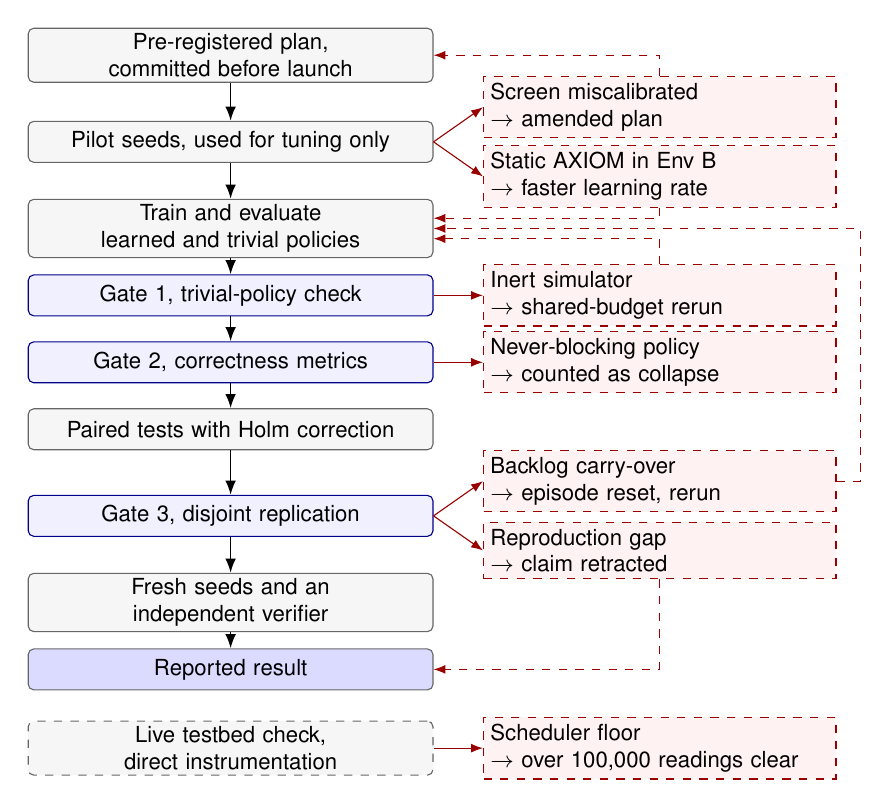
\begin{tikzpicture}[
  font=\figfont, x=1cm, y=1cm,
  every node/.append style={execute at begin node={\hyphenpenalty=10000\exhyphenpenalty=10000}},
  st/.style={draw=black!60, fill=gray!7, rounded corners=2pt, align=center, text width=5.0cm, minimum height=0.52cm, inner sep=2pt},
  gate/.style={st, draw=blue!55!black, fill=blue!6},
  fail/.style={draw=red!60!black, fill=red!5, dashed, align=left, text width=4.3cm, minimum height=0.52cm, inner sep=2.5pt},
  ar/.style={-{Latex[length=1.8mm]}, semithick},
  ct/.style={-{Latex[length=1.5mm]}, red!60!black},
  fb/.style={-{Latex[length=1.5mm]}, red!60!black, dashed}
]
% the protocol, top to bottom
\node[st]   (p1) at (2.65,0.00) {Pre-registered plan, committed before launch};
\node[st]   (p2) at (2.65,-1.10) {Pilot seeds, used for tuning only};
\node[st]   (p3) at (2.65,-2.20) {Train and evaluate learned and trivial policies};
\node[gate] (p4) at (2.65,-3.05) {Gate 1, trivial-policy check};
\node[gate] (p5) at (2.65,-3.90) {Gate 2, correctness metrics};
\node[st]   (p6) at (2.65,-4.75) {Paired tests with Holm correction};
\node[gate] (p7) at (2.65,-5.85) {Gate 3, disjoint replication};
\node[st]   (p8) at (2.65,-6.95) {Fresh seeds and an independent verifier};
\node[st, fill=blue!14] (p9) at (2.65,-7.80) {Reported result};
\foreach \a/\b in {p1/p2,p2/p3,p3/p4,p4/p5,p5/p6,p6/p7,p7/p8,p8/p9}{\draw[ar] (\a) -- (\b);}
% failures, each beside the step that caught it
\node[fail] (f1) at (8.10,-0.66) {Screen miscalibrated\\ $\rightarrow$ amended plan};
\node[fail] (f2) at (8.10,-1.54) {Static AXIOM in Env B\\ $\rightarrow$ faster learning rate};
\node[fail] (f3) at (8.10,-3.05) {Inert simulator\\ $\rightarrow$ shared-budget rerun};
\node[fail] (f4) at (8.10,-3.90) {Never-blocking policy\\ $\rightarrow$ counted as collapse};
\node[fail] (f5) at (8.10,-5.41) {Backlog carry-over\\ $\rightarrow$ episode reset, rerun};
\node[fail] (f6) at (8.10,-6.29) {Reproduction gap\\ $\rightarrow$ claim retracted};
\draw[ct] (p2.east) -- (f1.west);
\draw[ct] (p2.east) -- (f2.west);
\draw[ct] (p4.east) -- (f3.west);
\draw[ct] (p5.east) -- (f4.west);
\draw[ct] (p7.east) -- (f5.west);
\draw[ct] (p7.east) -- (f6.west);
% each failure changed an earlier step, or withdrew a claim
\draw[fb] (f1.north) |- (p1.east);
\draw[fb] (f2.south) |- ([yshift=1.3mm]p3.east);
\draw[fb] (f3.north) |- ([yshift=-1.3mm]p3.east);
\draw[fb] (f5.east) -- ++(0.3,0) |- (p3.east);
\draw[fb] (f6.south) |- (p9.east);
% the live testbed check
\node[st, dashed] (lv) at (2.65,-8.80) {Live testbed check, direct instrumentation};
\node[fail] (f7) at (8.10,-8.80) {Scheduler floor\\ $\rightarrow$ over 100{,}000 readings clear};
\draw[ct] (lv) -- (f7);
\end{tikzpicture}
\end{document}
